\documentclass[9pt, aspectratio=169]{beamer}
\usepackage{FiraSans}
\usetheme[subsectionpage=progressbar]{metropolis}
\usepackage[utf8]{inputenc}
\usepackage{amsmath}
\usepackage{amsfonts}
\usepackage{amssymb}
\usepackage{multicol}
\usepackage{tikz}
\usetikzlibrary{math, calc}
\usepackage{caption}
\usepackage{xcolor}
\usepackage[T1]{fontenc} 
\usepackage[skins]{tcolorbox}
\author{Nicola Roman\`o - nicola.romano@ed.ac.uk}
\title{Lecture 08 - Complex pipelines in image analysis}
\subtitle{Tracing, tracking and registration}
\setlength{\fboxsep}{0pt}
\setbeamertemplate {footline}{\begin{scriptsize}\hfill\insertframenumber ~of \inserttotalframenumber\kern1em\vskip5pt\end{scriptsize}}

% Remove "Figure" in front of captions
% See https://tex.stackexchange.com/questions/82456/how-to-remove-figure-caption-prefix-figure-in-beamer
\captionsetup{labelformat=empty,labelsep=none}

\titlegraphic{\centering \includegraphics[scale=.5]{instituteLogo.png}}
\date{}

\begin{document}

\newtcolorbox{codebox}{enhanced,
    top=2pt,
    left=2pt,
    right=2pt,
    bottom=2pt,
    boxrule=0pt,
    leftrule=5pt,
    sharp corners,
    colback=gray!20,
    colframe=blue!60!black}

\begin{frame}
    \titlepage
\end{frame}

\section{Recap}

\begin{frame}
    {In the past lectures...}
    We have seen how to

    \begin{itemize}
        \item [\checkmark] Use Numpy, Matplotlib and Scikit-image to \textbf{display} and manipulate images
        \item [\checkmark] \textbf{Preprocess images}, e.g. by modifying their histograms, or by using convolutional filters. This allows us to enhance contrast, sharpen or blur the image, find edges, etc.
        \item [\checkmark] Use \textbf{morphological operators} to perform image processing, e.g. erosion, dilation, opening, closing, etc.
        \item [\checkmark] \textbf{Extract features} from an image, to be used for further processing (blob, lines, circles, texture...)
        \item [\checkmark] \textbf{Segment} an image into different regions, e.g. by thresholding, clustering, watershed, etc.
    \end{itemize}
\end{frame}

\begin{frame}
    {In this lecture...}
    We are going to put all of this together today to see how we can perform more complex image processing.

    We are going to focus on three example tasks:

    \begin{itemize}
        \item [\checkmark] \textbf{Tracing} a structures in an image
        \item [\checkmark] \textbf{Tracking} a moving object in a sequence of images
        \item [\checkmark] \textbf{Registration} of images
    \end{itemize}

    \small
    \textit{Note}: this lecture will not go in depth into the details of the implementation of these tasks, but aims to give you an idea of how to build a pipeline to perform them using the tools we have seen so far.
\end{frame}

\begin{frame}
    {Learning objectives}
    \begin{columns}
        \begin{column}{0.8\textwidth}
            \begin{itemize}
                \item Describe the issues associated with tracing tube-like structures
                \item Describe pipelines for extracting information from these datasets.
                \item Describe strategies to track objects in a sequence of images
                \item Describe strategies to register images
            \end{itemize}
        \end{column}
        \begin{column}{0.2\textwidth}
            
\includegraphics[angle=-30, origin=tr, width=1.5\textwidth]{lightbulb.png}
        \end{column}
    \end{columns}
\end{frame}

\section{Tracing}

\begin{frame}
    {What is tracing?}
    \begin{columns}
        \begin{column}{.7\textwidth}
            In biomedical imaging, \textbf{tracing} is the process of segmenting tube-like structures in images.
            \vspace{1em}

            Note: some literature calls this tracking (e.g. vessel tracking), which should not be confused with motion tracking.
            \vspace{1em}

            This is often applied to blood vessels and neuronal processes.
        \end{column}
        \begin{column}{.3\textwidth}
            \includegraphics[width=\textwidth]{Babin2018-aneurysm.png}
            \footnotesize
            Babin et al. 2018 - Arteriovenous malformation in the brain.
        \end{column}
    \end{columns}
\end{frame}

\begin{frame}
    {Challenges}
    \begin{itemize}
        \item Complex morphologies
        \item Often need to work in 3D
        \item Can require a lot of computational power
    \end{itemize}
    \centering
    \includegraphics[width=.6\textwidth]{Boldog2018-neurons.png}

    \footnotesize
    Boldog et al. 2018 - 3D reconstruction of rosehip neurons in the human brain.

\end{frame}

\begin{frame}
    {Detecting blood vessels}
    \begin{columns}
        \begin{column}{.5\textwidth}
            Vessels can be characterised by colour, gradient, and contrast.
            \vspace{1em}

            Simple segmentation strategies are sub-optimal.
        \end{column}
        \begin{column}{.5\textwidth}
            \centering
            \includegraphics[width=\textwidth]{retina_thresholding.png}

            \footnotesize
            \raggedright
            Source: Mikael H\"aggstr\"om 2014, Fundus photograph of a normal right eye.
        \end{column}
    \end{columns}
\end{frame}

\begin{frame}
    {Filtering with morphological operators}
    Morphological operators can be often used to improve the image before thresholding.

    For example, \textbf{bottom-hat filtering} has been often used to help in segmenting blood vessels.

    \pause

    It involves applying a morphological closing to the image and then subtracting the original image from the result.
    By using a structural element larger than the structures of interest, we can isolate them from the image.

    \centering
    \includegraphics[width=.7\textwidth]{bh_example.png}

    \pause
    \small
    \begin{itemize}
        \item Bottom-hat filtering extracts objects \textbf{darker} than the background.
        \item Lighter objects can be extracted using \textbf{top-hat filtering}
        \item For top-hat, you subtract a morphological opening of the image from the original image itself.
    \end{itemize}
\end{frame}

\begin{frame}
    {Bottom-hat filtering of blood vessels}
    \centering
    \includegraphics[width=\textwidth]{retina_bottomhat.png}
\end{frame}
\begin{frame}
    {Template matching}
    \textbf{Template matching} allows finding small parts of an image matching a template image. The cross-correlation between the template and the image is calculated pixel-wise and the maxima are taken as matches.

    \only<1>{
        \includegraphics[width=\textwidth]{template_matching_Thomas_and_Gehrig.png}
        \footnotesize
        Thomas and Gehrig, 2020 - Template matching (followed by non-maxima suppression) to identify fish embryos in a plate.
    }

    \pause
    Template matching can be used for blood vessel detection by assuming that the cross section of the vessels is approximated by a Gaussian.

    \pause
    We design a series of templates, at various angles for piece-wise detection (in pieces of length L).

    $$K(x, y) = - e^{\frac{-x^2}{2*\sigma_x^2}}\qquad \text{for}~|y| \leq \frac{L}{2}$$

    \centering
    \includegraphics[width=.9\textwidth]{template_matching_kernels.png}
\end{frame}

\begin{frame}
    {Skeletonization}
    Skeletonization, or center-line extraction is an useful morphological operation that can help delineating tube-like structures in images.

    It works by thinning the image repeatedly until no more thinning is possible.

    \centering
    \includegraphics[width=.8\textwidth]{template_matching and skeleton.png}

    \footnotesize
    Green channel $\rightarrow$ bottom-hat filtering $\rightarrow$ template matching $\rightarrow$ remove small objects $\rightarrow$ skeletonization.
\end{frame}

\begin{frame}
    {From skeleton to graphs and features}

    Skeletonization can be mapped to a graph, a mathematical structure which allows for easier analysis of the structure.

    Features can be extracted to find vessel length, number and location of branching points, tortuosity, discriminate arteries and veins etc

    HOG features can be used to find the direction and bifurcation points of vessels.

    \includegraphics[width=\textwidth]{vesselHOG.png}

    \footnotesize
    Srinidhi, 2017
\end{frame}

\begin{frame}
    {Classification of intersections}
    Other than HOG features, other strategies have been used for classifying structural features of a vascular network. For example, detection of key-points followed by polar projection has been used to classify branches.

    \centering
    \includegraphics[width=.7\textwidth]
    {polar_map_classification_intersections.png}

    \footnotesize
    \raggedright
    Srinidhi, 2017
\end{frame}

\begin{frame}
    {Example of a complete pipeline}
    \centering
    \includegraphics[width=.8\textwidth]{retina_pipeline.png}

    \footnotesize
    Srinidhi et al. 2109 - extracting colour and other features allows for discrimination of arteries and veins.
\end{frame}

\section{Registration and motion tracking}
\begin{frame}
    {Reminder from lecture 1...}
    A video is just a sequence of images, that we can store in a tensor with 3 or more dimensions.

    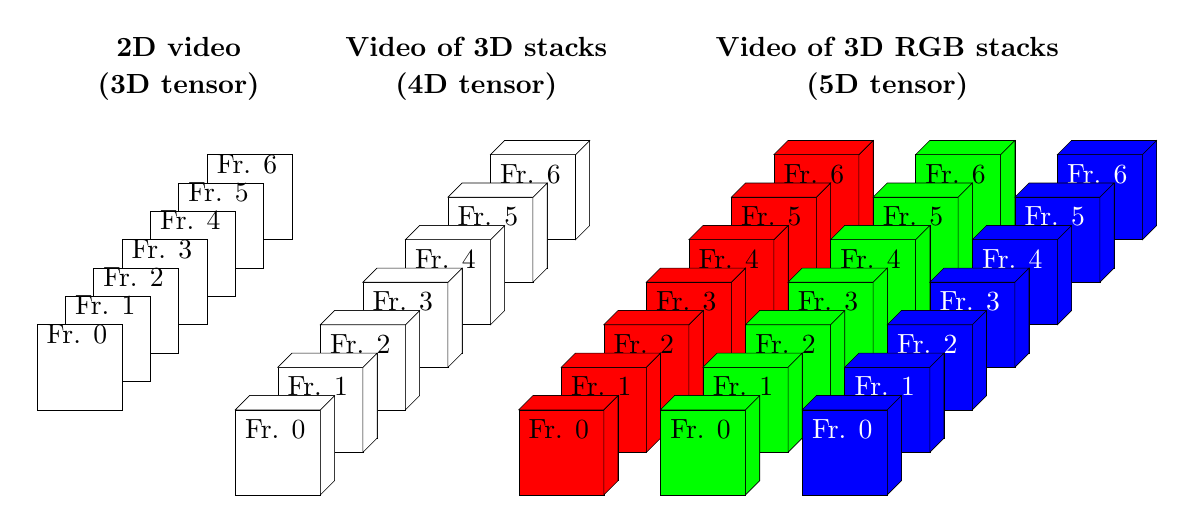
\begin{tikzpicture}[scale=.9]
        \foreach \i [count=\n] in {-1,-0.6,...,1.4}
            {
                \node (A) at ({-\i+1.2}, {-\i+1.2}) {};
                \node (B) at ({-\i}, {-\i}) {};

                \draw[black,very thin, fill=white] (A) rectangle (B);
                \tikzmath{\frame = int(7-\n);}
                \node[anchor=south west] at (-\i, -\i+.8) {Fr. \frame};
            }

        \foreach \i [count=\n] in {-1,-0.4,...,3}
            {
                %   G----A
                %  /|   / |
                % H-----C |
                % | B---|-E
                % |/    |/
                % D-----F
                \node (A) at (-\i+5.4, -\i+1.4) {};
                \node (B) at (-\i+4.2, -\i+0.2) {};
                \node (C) at (-\i+5.2, -\i+1.2) {};
                \node (D) at (-\i+4, -\i) {};
                \node (E) at (-\i+5.4, -\i+0.2) {};
                \node (F) at (-\i+5.2, -\i) {};
                \node (G) at (-\i+4.2, -\i+1.4) {};
                \node (H) at (-\i+4, -\i+1.2) {};

                % Back of the 3D stack
                \draw[black,very thin, fill=white] (A) rectangle (B);
                % Front of the 3D stack
                \draw[black,very thin, fill=white] (C) rectangle (D);
                % Side of the 3D stack
                % See https://tex.stackexchange.com/questions/4057/cycle-option-when-drawing-between-nodes-in-tikz
                % for the explanation of .center
                \draw[black,very thin, fill=white] (A.center) -- (E.center) -- (F.center) -- (C.center) -- cycle;
                % Top of the 3D stack
                \draw[black,very thin, fill=white] (A.center) -- (G.center) -- (H.center) -- (C.center) -- cycle;

                % Draw the frame number
                \tikzmath{\frame = int(7-\n);}
                \node[anchor=north west] at (H) {Fr. \frame};
            }


        \foreach \i [count=\n] in {-1,-0.4,...,3}
            {
                %   G----A
                %  /|   / |
                % H-----C |
                % | B---|-E
                % |/    |/
                % D-----F
                \node (A) at (-\i+9.4, -\i+1.4) {};
                \node (B) at (-\i+8.2, -\i+0.2) {};
                \node (C) at (-\i+9.2, -\i+1.2) {};
                \node (D) at (-\i+8, -\i) {};
                \node (E) at (-\i+9.4, -\i+0.2) {};
                \node (F) at (-\i+9.2, -\i) {};
                \node (G) at (-\i+8.2, -\i+1.4) {};
                \node (H) at (-\i+8, -\i+1.2) {};

                % Red channel
                % Back of the 3D stack
                \draw[black,very thin, fill=red] (A) rectangle (B);
                % Front of the 3D stack
                \draw[black,very thin, fill=red] (C) rectangle (D);
                % Side of the 3D stack
                % See https://tex.stackexchange.com/questions/4057/cycle-option-when-drawing-between-nodes-in-tikz
                % for the explanation of .center
                \draw[black,very thin, fill=red] (A.center) -- (E.center) -- (F.center) -- (C.center) -- cycle;
                % Top of the 3D stack
                \draw[black,very thin, fill=red] (A.center) -- (G.center) -- (H.center) -- (C.center) -- cycle;

                % Green channel
                % Back of the 3D stack
                \draw[black,very thin, fill=green] ($(A) + (2, 0)$) rectangle ($(B) + (2, 0)$);
                % Front of the 3D stack
                \draw[black,very thin, fill=green] ($(C) + (2, 0)$) rectangle ($(D) + (2, 0)$);
                % Side of the 3D stack
                % See https://tex.stackexchange.com/questions/4057/cycle-option-when-drawing-between-nodes-in-tikz
                % for the explanation of .center
                \draw[black,very thin, fill=green] ($(A.center) + (2, 0)$) -- ($(E.center) + (2, 0)$) -- ($(F.center) + (2, 0)$) -- ($(C.center) + (2, 0)$) -- cycle;
                % Top of the 3D stack
                \draw[black,very thin, fill=green] ($(A.center) + (2, 0)$) -- ($(G.center) + (2, 0)$) -- ($(H.center) + (2, 0)$) -- ($(C.center) + (2, 0)$) -- cycle;

                % Blue channel
                % Back of the 3D stack
                \draw[black,very thin, fill=blue] ($(A) + (4, 0)$) rectangle ($(B) + (4, 0)$);
                % Front of the 3D stack
                \draw[black,very thin, fill=blue] ($(C) + (4, 0)$) rectangle ($(D) + (4, 0)$);
                % Side of the 3D stack
                % See https://tex.stackexchange.com/questions/4057/cycle-option-when-drawing-between-nodes-in-tikz
                % for the explanation of .center
                \draw[black,very thin, fill=blue] ($(A.center) + (4, 0)$) -- ($(E.center) + (4, 0)$) -- ($(F.center) + (4, 0)$) -- ($(C.center) + (4, 0)$) -- cycle;
                % Top of the 3D stack
                \draw[black,very thin, fill=blue] ($(A.center) + (4, 0)$) -- ($(G.center) + (4, 0)$) -- ($(H.center) + (4, 0)$) -- ($(C.center) + (4, 0)$) -- cycle;

                % Draw the frame number
                \tikzmath{\frame = int(7-\n);}
                \node[anchor=north west] at (H) {Fr. \frame};
                \node[anchor=north west] at ($(H) + (2,0)$) {Fr. \frame};
                \node[anchor=north west] at ($(H) + (4,0)$) {\color{white}{Fr. \frame}};
            }

        \node [anchor=north] at (.6, 4) {\textbf{2D video}};
        \node [anchor=north] at (.6, 3.5) {\textbf{(3D tensor)}};

        \node [anchor=north] at (4.8, 4) {\textbf{Video of 3D stacks}};
        \node [anchor=north] at (4.8, 3.5) {\textbf{(4D tensor)}};

        \node [anchor=north] at (10.6, 4) {\textbf{Video of 3D RGB stacks}};
        \node [anchor=north] at (10.6, 3.5) {\textbf{(5D tensor)}};

    \end{tikzpicture}
\end{frame}

\begin{frame}
    {Videos in biomedical imaging}
    \begin{itemize}
        \item Many biological processes are dynamic and capturing/analysing them is a challenging task.
        \item Often tradeoff between acquisition speed and image quality is needed.
        \item Need analysis methods that are robust to noise and outliers.
        \item Generally we want to find object(s) of interest in each frame and be able to identify them across frames.
    \end{itemize}
\end{frame}

\begin{frame}
    {Some examples}
    Examples of dynamic biological processes captured in videos.
    \begin{itemize}[<+->]
        \item Tracking single molecules, vesicles, organelles in a cell
        \item Tracking cells in a dish or in a tissue
        \item Tracking a mouse during a behavioural experiment
    \end{itemize}

    \centering
    \only<1>{
        \includegraphics[width=.5\textwidth]{Choquet_Triller_2003_single_molecule_tracking.png}

        \footnotesize
        Choquet and Triller, 2003 - Tracking of AMPA receptors on a cell.
    }
    \only<2>{
        \includegraphics[width=.5\textwidth]{Perkin_Elmer_cell_tracking.jpg}

        \footnotesize
        Perkin Elmer - Tracking of cells in a dish.
    }
    \only<3>{
        \includegraphics[width=.7\textwidth]{Zhang_2020_mouse_tracking.png}

        \footnotesize
        Mouse tracking in a behavioural experiment.
    }
\end{frame}

\begin{frame}
    {A general motion tracking pipeline}

    \begin{enumerate}
        \item (\textit{optional}) Registration of the video
        \item Object detection
        \item Object tracking
        \item Measurement of object properties over time
    \end{enumerate}
\end{frame}

\section{Registration}

\begin{frame}
    {Registration}
    Registration (or video stabilization) is the process of aligning the video frames to a reference frame; this is done to correct for the movement of the camera or of the sample.
    \pause

    For instance, registration is useful for correcting:

    \begin{itemize}
        \item In vivo imaging where breathing artefacts can shift the field of view
        \item Drifting of the sample under a microscope
        \item Aligning MRI from the same subject in different sessions
    \end{itemize}
\end{frame}

\begin{frame}
    {Registration - motivation}
    Registration is important because otherwise quantification could be inaccurate.

    \centering
    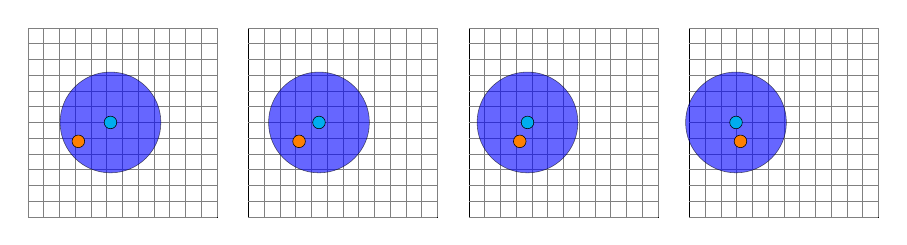
\begin{tikzpicture}[scale=.8]
        \foreach \i [count=\n] in {0,3.5,7,10.5}
            {
                \draw[black,very thin, fill=white] (\i, 0) rectangle ({\i+3}, 3);
                \draw[gray,very thin, step=.25] (\i, 0) grid ({\i+3}, 3);

                \draw[black,very thin, fill=blue, opacity=0.6] ({\i+1.5+\n*(-0.19)}, 1.5) circle (0.8);
                \node (cellA) at ({\i+1.5+\n*(-0.19)}, 1.5) {};
                \node (cellB) at ({0.8+\i*1.001},{1.2}) {};
                \draw[very thin, fill=cyan] (cellA) circle (0.1);
                \draw[very thin, fill=orange] (cellB) circle (0.1);
            }
    \end{tikzpicture}

    \raggedright
    The orange cell is moving horizontally to the right, while the cyan cell is fixed; because the coverslip is drifting to the left, the coordinates of the orange cell stay fixed, while the cyan cell appers to move to the left.

    \pause
    While it is relatively straightforward to correct for this drift, drift in the z-axis is much more complex, as it changes the plane of focus that is being imaged.
\end{frame}

\begin{frame}
    {Types of registration algorithms}
    We can classify registration algorithms into

    \begin{itemize}
        \item \textbf{Intensity-based} - compare intensity patterns between the reference and the current frame via correlation
        \item \textbf{Feature-based} - find correspondences between features (points, corners etc) in the reference and the current frame
        \item \textbf{Mixed approaches}
    \end{itemize}

    \pause
    Registration can be performed through:

    \begin{itemize}
        \item \textbf{Rigid-body transformations} - translations and rotations only
        \item \textbf{Non-linear transformations} - including affine transformations (scaling, shearing)perspective transformations, curved transformations etc
    \end{itemize}
\end{frame}

\begin{frame}
    {Rigid-body registration}
    \textbf{Rigid-body} transformation is the simplest form of registration, consisting only of \textbf{translations and rotations}.

    Remember from Lecture 2:

    \centering
    \textbf{Translation}
    $$\begin{bmatrix}x'\\y'\\1\end{bmatrix} = \begin{bmatrix}1&0&t_x\\0&1&t_y\\0&0&1\end{bmatrix}\begin{bmatrix}x\\y\\1\end{bmatrix}$$
    \textbf{Rotation}
    $$\begin{bmatrix}x'\\y'\\1\end{bmatrix} = \begin{bmatrix}\text{cos}\theta&-\text{sin}\theta&0\\\text{sin}\theta&\text{cos}\theta&0\\0&0&1\end{bmatrix}\begin{bmatrix}x\\y\\1\end{bmatrix}$$
    % \textbf{Scaling}
    % $$\begin{bmatrix}x'\\y'\\1\end{bmatrix} = \begin{bmatrix}s_x&0&0\\0&s_y&0\\0&0&1\end{bmatrix}\begin{bmatrix}x\\y\\1\end{bmatrix}$$
\end{frame}

\begin{frame}
    {Rigid-body registration process}
    We want to find a transformation (translation+rotation) that maps the reference frame to the current frame.

    For \textbf{intensity-based registration}, given a frame at time $t$ and a reference frame at time $t_1$, we can find the offset $(u,v)$ that minimizes the MSE:

    \Large
    $$(u,v) = \underset{(u,v)}{\text{argmin}}\sum_x\sum_y(I_{i-1}(x,y)-I_{i}(x-u, y-v))^2$$

    \normalsize
    Alternatively, one could maximise the correlation between the two frames:

    \Large
    $$(u,v) = \underset{(u,v)}{\text{argmax}}\sum_x\sum_y(I_{i-1}(x,y)\cdot I_{i}(x-u, y-v))^2$$
\end{frame}

\begin{frame}
    {Registration - example}
    \includegraphics[width=\textwidth]{Lorenz2013_registration.png}

    \footnotesize
    Maximum intensity projection (over the time axis) of a video of kidney vascular flow. Rigid body registration is used to correct for the drift of the sample.
\end{frame}

\begin{frame}
    {Feature-based registration}
    Feature-based registration is based on the idea that there are static features in the video, that can be used to match images from one frame to another.
    \centering
    \includegraphics[width=.5\textwidth]{Alam2017_registration.png}

    \footnotesize
    Feature-based non-linear registration of brain MRI images.
\end{frame}
\section{Object detection and tracking}

\begin{frame}
    {Object detection}
    Object detection in a video is the same process than in a single image.

    All the segmentation techniques we have seen so far are applicable in this case as well!
\end{frame}

\begin{frame}
    {Object tracking}
    Once we found the object(s) of interest in each frame we want to be able to track them over time.

    That is, given $n$ object in a frame, $O_1, O_2, \ldots, O_n$ and $n$ we want to match each of them to the same object in the previous frame.
\end{frame}

\begin{frame}
    {Nearest-neighbour traking}
    If the objects are spaced far apart and do not make large movements from frame to frame, we can use a \textbf{nearest-neighbour} approach.

    \pause

    \begin{itemize}
        \item For each detected object we create a window of size $w$ containing it.
        \item We find the object in the next frame that is closest to the object of interest within that window.
              \pause
        \item Improved by predicting the position of the window surrounding the object, based on the displacement in previous frames
        \item The window could be expanded if no object is found.
    \end{itemize}
\end{frame}

\begin{frame}
    {Greedy algorithms}
    Nearest-neighbour tracking can only handle simple situations. For example, it fails if the object disappears for a certain time.

    In this case, we can use a \textbf{greedy algorithm} instead.

    \begin{itemize}[<+->]
        \item For each object $O$ in frame $n$ we define a window surrounding it.
        \item We look in frame $n+1$ for any object in the window.
        \item We score each object according to a metric (e.g. intensity correlation, or position).
        \item We select the object with the highest score and keep it as a match.
        \item If subsequent frames contradict the match, we step back and take the second best object.
        \item We can also add dummy object with a score of zero, which we can use as placeholders for disappearing objects (either ending that track or "putting it on hold" until it reappears).
    \end{itemize}

    \pause
    This type of algorithm works well with relatively sparse and slow moving objects.
\end{frame}

\begin{frame}
    {Histogram tracking}
    Another popular algorithm is the \textbf{mean-shift} algorithm.

    \begin{itemize}[<+->]
        \item We compute the histogram for our object of interest
        \item We then "back-project" the histogram onto the new frame. This means that we take each pixel in the search window and sum the probability of their intensities in the histogram.
        \item We then try to maximise this probability by shifting the search window. 
    \end{itemize}
\end{frame}
\section {Measurement of object properties}

\begin{frame}
    {Measuring cell properties}
    Just as we saw in the segmentation lecture we can use the \texttt{regionprops} function to measure properties of the detected objects.

    We will simply measure these properties in each frame by applying the function multiple times.
    
    Furthermore knowing the position of the object(s) in each frame we can calculate their direction and speed. 
\end{frame}


\end{document}

